\chapter{ユーザインターフェース}
\section{画面遷移}
画面遷移図は,\figref{fig:管理者側画面遷移図},\figref{fig:ユーザ側画面遷移図}の通りである.
\begin{figure}[H]
    \centering
    \begin{framed}
        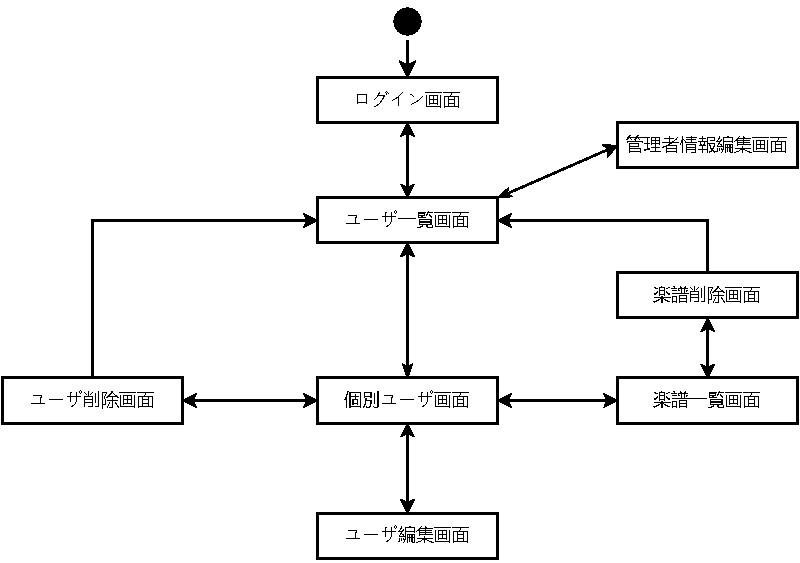
\includegraphics[keepaspectratio,width=\textwidth]{ui/管理者側画面遷移図.pdf}
    \end{framed}
    \caption{管理者側画面遷移図}
    \label{fig:管理者側画面遷移図}
\end{figure}
\begin{figure}[H]
    \begin{framed}
        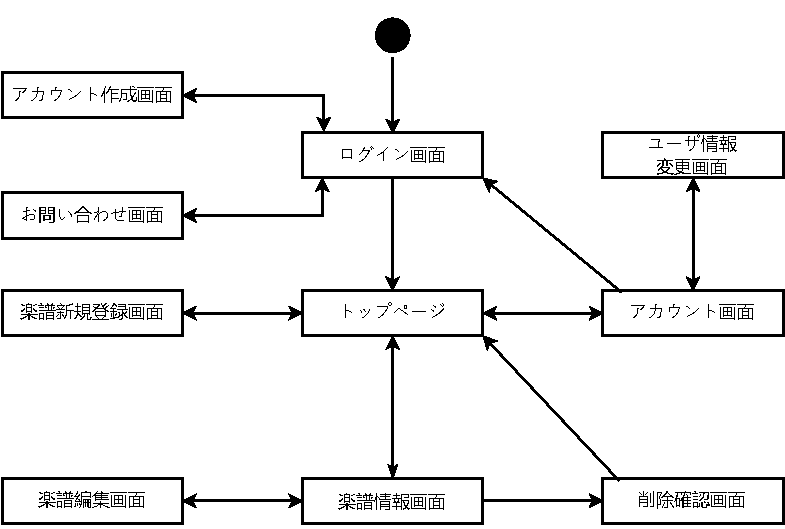
\includegraphics[keepaspectratio,width=\textwidth]{ui/ユーザ側画面遷移図.pdf}
    \end{framed}
    \caption{ユーザ側画面遷移図}
    \label{fig:ユーザ側画面遷移図}
\end{figure}
\section{UI View}
\subsection*{ユーザ側UI(→p.\pageref{fig:ui-view:user}〜)}
\subsection*{管理者側UI(→p.\pageref{fig:ui-view:admin}〜)}
「ログイン」は,ユーザ側UIと共通のため,p.\pageref{fig:ui-view:user}に記載している.
\newcommand{\vuser}[4]{\begin{figure}[H]\centering\begin{minipage}[b]{.48\textwidth}\centering\includegraphics[keepaspectratio,width=\textwidth]{ui/user/#1.png}\caption{#2}\end{minipage}\begin{minipage}[b]{.48\textwidth}\centering\includegraphics[keepaspectratio,width=\textwidth]{ui/user/#3.png}\caption{#4}\end{minipage}\end{figure}}
\vuser{0-ログイン}{ログイン}{1-利用登録}{利用登録}\label{fig:ui-view:user}
\vuser{2-トップページ画面}{トップページ}{3-楽曲登録:編集}{楽譜登録,編集}
\vuser{4-マイページ}{マイページ}{10-楽曲操作決定}{楽譜詳細画面}
\vuser{5-楽曲編集確認}{楽曲編集}{7-ユーザパスワード変更}{パスワード変更}
\vuser{7-ユーザ情報編集}{ユーザ情報編集}{7-ユーザ情報編集エラー}{ユーザ情報編集エラー}
\vuser{8-ユーザ情報削除確認}{ユーザ情報削除確認}{9-お問い合わせ}{お問合せ画面}
\newcommand{\vadmin}[4]{\begin{figure}[H]\centering\begin{minipage}[b]{.48\textwidth}\centering\includegraphics[keepaspectratio,width=\textwidth]{ui/admin/#1.png}\caption{#2}\end{minipage}\begin{minipage}[b]{.48\textwidth}\centering\includegraphics[keepaspectratio,width=\textwidth]{ui/admin/#3.png}\caption{#4}\end{minipage}\end{figure}}
\vadmin{0-トップページ}{トップページ}{1-操作選択}{操作選択}\label{fig:ui-view:admin}
\vadmin{2-ユーザ情報編集}{ユーザ情報編集}{2-ユーザ情報編集エラー}{ユーザ情報編集エラー}
\vadmin{2-ユーザ情報編集確認}{ユーザ情報編集確認}{3-ユーザ削除確認}{ユーザ削除確認}
\vadmin{4-ユーザ楽曲DB}{楽譜DB一覧}{4-ユーザ楽曲削除確認}{楽譜削除確認}
\vadmin{5-管理者情報編集}{管理者情報編集}{2-ユーザ情報編集エラー}{ユーザ情報編集エラー}